\documentclass[a4paper,12pt]{article} % добавить leqno в [] для нумерации слева
\usepackage[a4paper,top=1.3cm,bottom=2cm,left=1.5cm,right=1.5cm,marginparwidth=0.75cm]{geometry}
%%% Работа с русским языком
\usepackage{cmap}					% поиск в PDF
\usepackage[warn]{mathtext} 		% русские буквы в фомулах
\usepackage[T2A]{fontenc}			% кодировка
\usepackage[utf8]{inputenc}			% кодировка исходного текста
\usepackage[english,russian]{babel}	% локализация и переносы
\usepackage{physics}
\usepackage{multirow}

%%% Нормальное размещение таблиц (писать [H] в окружении таблицы)
\usepackage{float}
\restylefloat{table}


\usepackage{graphicx}

\usepackage{wrapfig}
\usepackage{tabularx}

\usepackage{hyperref}
\usepackage[rgb]{xcolor}
\hypersetup{
	colorlinks=true,urlcolor=blue
}

%%% Дополнительная работа с математикой
\usepackage{amsmath,amsfonts,amssymb,amsthm,mathtools} % AMS
\usepackage{siunitx}
\usepackage{icomma} % "Умная" запятая: $0,2$ --- число, $0, 2$ --- перечисление

%% Номера формул
%\mathtoolsset{showonlyrefs=true} % Показывать номера только у тех формул, на которые есть \eqref{} в тексте.

%% Шрифты
\usepackage{euscript}	 % Шрифт Евклид
\usepackage{mathrsfs} % Красивый матшрифт
\usepackage{pgfplots}
\pgfplotsset{compat=1.9}

%% Свои команды
\DeclareMathOperator{\sgn}{\mathop{sgn}}

%% Перенос знаков в формулах (по Львовскому)
\newcommand*{\hm}[1]{#1\nobreak\discretionary{}
	{\hbox{$\mathsurround=0pt #1$}}{}}

\date{\today}

\begin{document}

\begin{titlepage}
	\begin{center}
		{\large МОСКОВСКИЙ ФИЗИКО-ТЕХНИЧЕСКИЙ ИНСТИТУТ (НАЦИОНАЛЬНЫЙ ИССЛЕДОВАТЕЛЬСКИЙ УНИВЕРСИТЕТ)}
	\end{center}
	\begin{center}
		{\large Физтех-школа электроники, фотоники и молекулярной физики}
	\end{center}
	
	
	\vspace{4.5cm}
	{\huge
		\begin{center}
			{Лабораторная работа по химической физике}\\
                {"Изучение адсорбции ароматических соединений из водных растворов на активированных углях методом УФ-спектрометрии".}\\
		\end{center}
	}
	\vspace{2cm}
	\begin{flushright}
		{\LARGE Авторы:\\ Беляев Юрий \\ Борисов Павел \\ Фейзрахманов Эмир  \\
			\vspace{0.2cm}
			группа Б04-202}
	\end{flushright}
	\vspace{7.5cm}
	\begin{center}
		\today
	\end{center}
\end{titlepage}

\textbf{Цель работы: }
Получить изотермы адсорбции бензойной кислоты (БК) на углеродном адсорбенте и проанализировать их, используя уравнения Генри, Фрейндлиха, Ленгмюра.
\par
\bigskip
\textbf{Оборудование: }
\begin{itemize}
    \item мерные колбы на 100 мл - 6 шт.;
    \item конические колбы на 50 мл со стеклянными пробками - 6 шт.;
    \item лабораторный стакан на 250 мл - 1 шт.;
    \item стеклянная воронка - 1 шт.;
    \item бумажный фильтр - 6 шт.;
    \item пипетка на 25 мл. с делениями - 1 шт.;
    \item лабораторный шейкер ПЭ-0034;
    \item аналитические весы с разрешением 0,1 мг;
    \item УФ-спектрофотометр;
    \item кварцевые кюветы толщиной 1,0 см с крышечками - 2 шт.;
    \item сорбент: активный уголь;
    \item насыщенный раствор бензойной кислоты (БК) в мерной колбе - 1 л;
    \item хромовая смесь;
    \item дистиллированная вода;
    \item бумажные салфетки.
\end{itemize}
\section*{Теоретическое введение}
\subsection*{Адсорбционные равновесия}
Поглощение вещества поверхностью твердого тела из объемной жидкой или газовой фазы называют \textit{адсорбцией}, вещество на поверхности которого протекает адсорбция, - \textit{адсорбентом}, поглощенное вещество - \textit{адсорбантом}, а вещество в объемной фазе - \textit{адсорбтивом} (рис.\ref{AD}). Иногда используются термины \textit{сорбция, сорбент, сорбат, сорбтив}.
\begin{figure}[H]
  \begin{minipage}[c]{0.5\textwidth}
    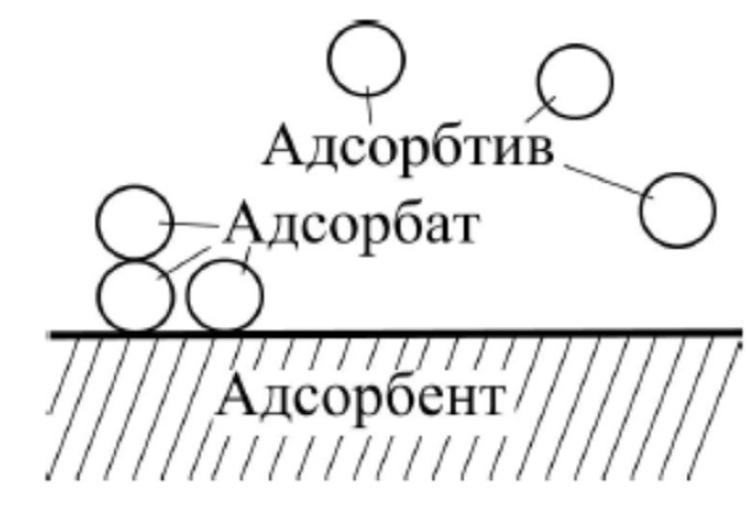
\includegraphics[width=10cm]{adsorb.png}
  \end{minipage}\hfill
  \begin{minipage}[c]{0.4\textwidth}
    \caption{
       Модель процесса адсорбции.
    } \label{AD}
  \end{minipage}
\end{figure}
\par
Адсорбция носит динамический характер, т.е. равновесие в системе достигается, когда скорость десорбции становится равной скорости адсорбции.
\subsection*{Методы и уравнения для описания адсорбции}
Количество адсорбированного вещества и сопровождающие адсорбцию тепловые эффекты зависят от свойств адсорбтива, адсорбента, а также от температуры, давления и концентрации адсорбируемого вещества. Зависимость адсорбции от давления газа или концентрации вещества в растворе при постоянной температуре описывается \textit{изотермой адсорбции}. Для её построения применяют уравнения, учитывающие однородность или неоднородность поверхности адсорбента и строение слоя адсорбента.
\par
 Получим некоторые из этих уравнений. В табл. \ref{vel} приведены общепринятые обозначения, которые мы будем использовать.
\begin{table}[H]
\centering 
    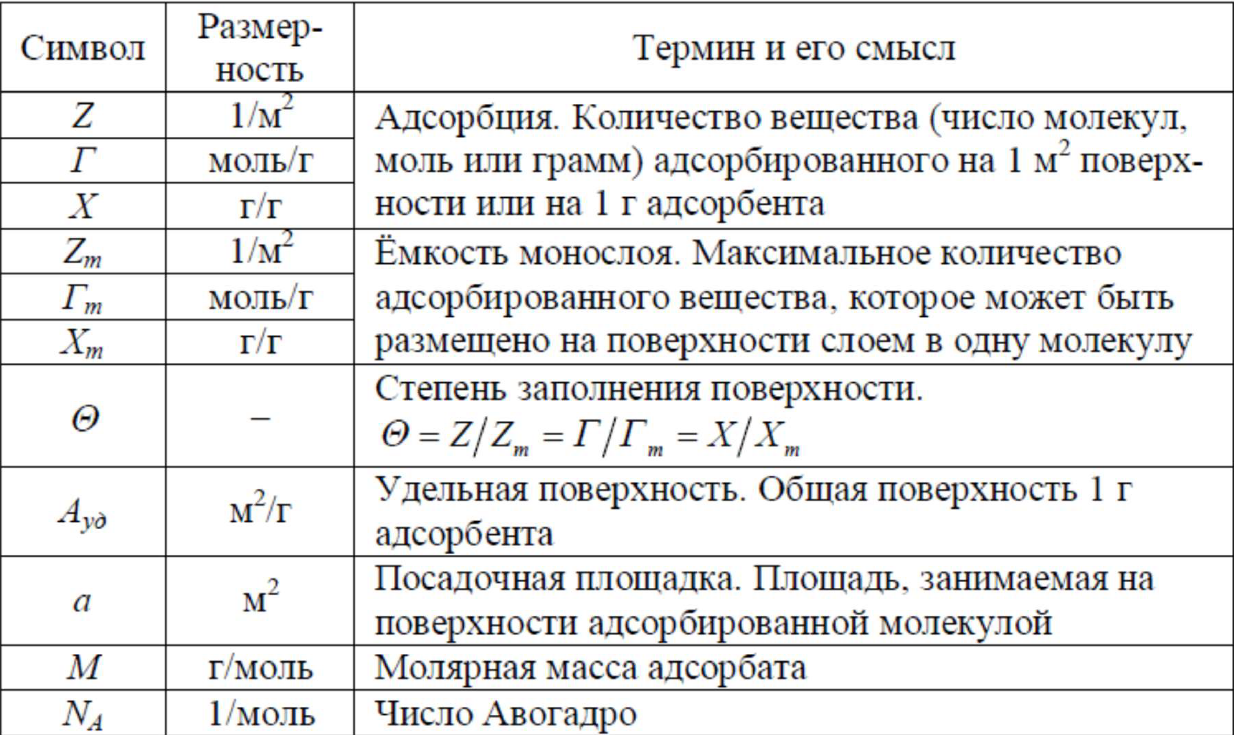
\includegraphics[width=15cm]{vel.png}
    \caption{Общепринятые обозначения.}
    \label{vel}
\end{table}
\subsection*{Изотермы Ленгмюра и Генри}
Предположим, что поверхность адсорбента однородна, адсорбат распологается на поверхности слоем в одну молекулу и взаимодействием между адсорбированными молекулами можно пренебречь. Тогда весь процесс будет описываться схемой:
\begin{equation*}
    M + () \rightleftarrows (M), \textrm{ где}
\end{equation*}
$M$ - молекула адсорбтива, 
\newline 
$()$ - свободное место на поверхности адсорбента, 
\newline 
($M$) - адсорбированная молекула. 
\newline
Отсюда константа равновесия адсорбции $К$ находится по формуле:
\begin{equation*}
    K = \dfrac{Z}{(Z_m - Z)\cdot P} = \dfrac{\Theta}{(1 - \Theta)\cdot P},  \textrm{ где}
\end{equation*}
\newline $Z$, $Z_m$, $\Theta$ - см. в табл. \ref{vel}, 
\newline $(Z_m - Z)$ - количество свободных мест на границе адсорбента, 
\newline $P$ - равновесное давление адсорбтива над адсорбентом (бар). 
\newline Отсюда получаем уравнение:
\begin{equation}
    \Theta = \dfrac{K \cdot P}{1 + K \cdot P}.
    \label{eq:leng}
\end{equation}
Уравнение \eqref{eq:leng} называется \textit{изотермой Ленгмюра}.
\par
Перепишем уравнение \eqref{eq:leng} в более удобном виде:
\begin{equation*}
    \dfrac{1}{\Theta} = 1 + \dfrac{1}{K} \cdot \dfrac{1}{P}.
\end{equation*}
При $K \cdot P >> 1$ значение $\Theta \rightarrow 1$, т.е. к предельной степени заполнения при монослойной адсорбции.
При $K \cdot P << 1$ уравнение \eqref{eq:leng} переходит в \textit{изотерму Генри}:
\begin{equation}
    \Theta = K \cdot P.
    \label{eq:henry}
\end{equation}
Изотерма Генри описывает адсорбцию на однородной поверхности при малых заполнениях.

\subsection*{Изотерма Фрейндлиха}
Однако изотермы Ленгмюра и Генри часто расходятся с полученными эмпирическими методами результатами. Тогда Г. М. Фрейндлих предложил эмперическое уравнение для описания адсорбции, по которому количество адсорбированного вещества возврастает не пропорционально давлению, а заметно медленнее:
\begin{equation}
    \Gamma = K_\Phi \cdot P^n, \textrm{ где}
    \label{fr}
\end{equation}
$\Gamma$ - величина адсорбции (моль/г), 
\newline $P$ - равновесное давление адсорбтива (бар), 
\newline $K_\Phi$ - константа Фрейндлиха, 
\newline показатель степени $n \approx 0,1 - 0,7$.
\newline
Уравнение \eqref{fr} называется \textit{изотермой Фрейндлиха}, и оно хорошо описывает экспериментальные изотермы адсорбции на неоднородной поверхности в области средних заполнений. Часто уравнение \eqref{fr} переписывают в таком виде:
\begin{equation}
    \ln{\Gamma} = \ln K + n \ln P.
\end{equation}

\subsection*{Закон Бугера - Ламберта - Бера}
На практике для того чтобы количественно измерить адсорбцию в растворе пользуются законом  \textit{Бугера - Ламберта - Бера}, который определяет ослабление параллельного монохроматического пучка света при его распространении в поглощающей среде:
\begin{equation}
    I(l) = I_0 \cdot e^{-\varepsilon Cl}, \textrm{ где}
    \label{blb}
\end{equation}
  $l$ - длина кюветы, 
  \newline $C$ - концентрация светопоглощающего раствора, \newline $I_0$ - интенсивность света до прохождения через кювету, 
  \newline $\varepsilon$ - коэффициент экстинкции.
\newline
Преобразуем данный закон. Введем $D$ - оптическую плотность раствора:
\begin{equation}
    D := lg(\dfrac{I_0}{I}) \approx \varepsilon_{10}Cl,
\end{equation}
 Также справедливо равенство:
\begin{equation}
    D = \sum_{i}D_i= l \cdot \sum_{i}\varepsilon_iC_i, \textrm{ где}
    \label{add}
\end{equation}
$D_i$ - оптическая плотность компонент раствора, состоящего из невзаимодействующих веществ. 
\newline Cуммирование здесь ведется по всем компонентам раствора.
\par
В нашей работе с помощью спектрофотометра производились измерения оптической плотности $D$ в зависимости от длины волны $\lambda$. Затем посредством вычисленного коэффициента экстинкции можно вычислить концентрацию БК после адсорбции и как следствие найти величину адсорбции.

\subsection*{Анализ изотерм адсорбции веществ из растворов}
Для анализа изотерм адсорбции веществ из растворов чаще всего используют уравнения Фрейндлиха или Ленгмюра, а для анализа линейных изотерм - уравнение Генри. При этом в данных уравнениях давление паров адсорбтива в газовой фазе заменяют на концентрацию адсорбтива в растворе.
\par
Тогда новый вид уравнений Генри \eqref{eq:henry} и Фрейндлиха \eqref{fr} соответсвенно :
\begin{equation}
    \Gamma = K_H\cdot C, \quad \Gamma = K_\Phi \cdot C^n, \textrm { где}
\end{equation}
$\Gamma$ - величина адсорбции (моль/г), 
\newline $C$ - равновесная концентрация (моль/л), 
\newline $K_H$ - константа Генри,
\newline $K_\Phi$ - константа Фрейндлиха.
\newline Аналогично уравнение Ленгмюра \eqref{eq:leng} используют в форме:
\begin{equation}
    \Gamma = \Gamma_m\dfrac{K_LC}{1 + K_LC}, \quad \dfrac{1}{\Gamma} = \dfrac{1}{\Gamma_m} + \dfrac{1}{K_L \cdot \Gamma_m} \cdot \dfrac{1}{C}, \textrm{ где}
\end{equation}
$K_L$ - константа Ленгмюра.
\\
Используя полученные значения $\Gamma_m$ и $K_L$ можно вычислить максимальный объем $V_0$ адсорбированного вещества в рассчетет на единицу массы сорбента и площадь $\sigma$, которую занимает на поверхности одна молекула адсорбанта по формулам:
\begin{equation}
    V_0 =\dfrac{\Gamma_m \cdot M}{\rho}, \quad  a =\dfrac{A_{\text{уд}}}{\Gamma_m \cdot N_A}, \textrm{ где}
\end{equation}
$\rho$ - плотность конденсированной фазы адсорбтива, \newline $A_\text{уд}$ - удельная поверхность сорбента.
    


\section*{Ход работы}
\subsection*{Приготовление растворов}
Сначала в 6 мерных колбах на 100 мл. мы приготовили рабочие растворы БК путем разбавления ее насыщенного раствора с концентрацией 0,022 моль./л. (при $20^{\circ} C$) в следующих пропорциях (см табл. \ref{prop} в приложении).

\par
Затем в каждую из 6 конических колб на 50 мл. поместили навеску сорбента массой 0,033 г. и прилили по 30 мл. ранее приготовленных водных растворов БК разной концентрации.
Далее установили колбы на шейкер для равномерного встряхивания (на 1 час) растворов с адсорбентом при комнатной температуре. 

\subsection*{Запись спектров}
Запись спектров производилась с помощью непосредственно спектрофотометра и подключенного к нему компьютера. Сначала снимался спектр для дистиллированной воды, который впоследствии выбирался за "ноль" в диапазоне волн от 200 нм. до 400 нм.
\par
После установки "нуля" снимались спектры исходных растворов (без угля). Определялась оптическая плотность растворов с известной концентрации БК на максимуме второго пика поглощения (275 нм. - характерная длина волны поглощения ароматического кольца).
Затем аналогичная процедура измерениий производилась для растворов после адсорбции. Предварительно растворы были отфильтрованы бумажным фильтром от углеродного сорбента.





\subsection*{Обработка данных}
\textbf{Все последующие зависимости были аппроксимированы прямыми с помощью мнк. Для проверки гипотезы линейного закона вычислялся коэффициент корреляции Пирсона}.
\par
После измерения спектров на экране компьютера мы получали зависимость в виде графика $D(\lambda$), построенную с помощью интерфейса компьютера. Для начала убедились, что "ноль" в виде дистиллированной воды действительно записался и сняли повторно дистиллированную воду, но уже в режиме измерений (см. рис. \ref{wat} в приложении). Получили, что расхождения оптической плотности на всем спектре (200-400 нм.) не превышают \textbf{0.030}, а в пределах интересующего нас интервала 270-275 нм. $D$ не поднимается выше \textbf{0.010,} что гарантирует достаточно неплохую точность для дальнейших измерений с помощью спектрофотометра.
\par
Затем были получены спектры для 6 чистых растворов БК (см. рис. \ref{spec}) и для 6 растворов после адсорбции (см. рис. \ref{spec_}).

\begin{figure}[H]
    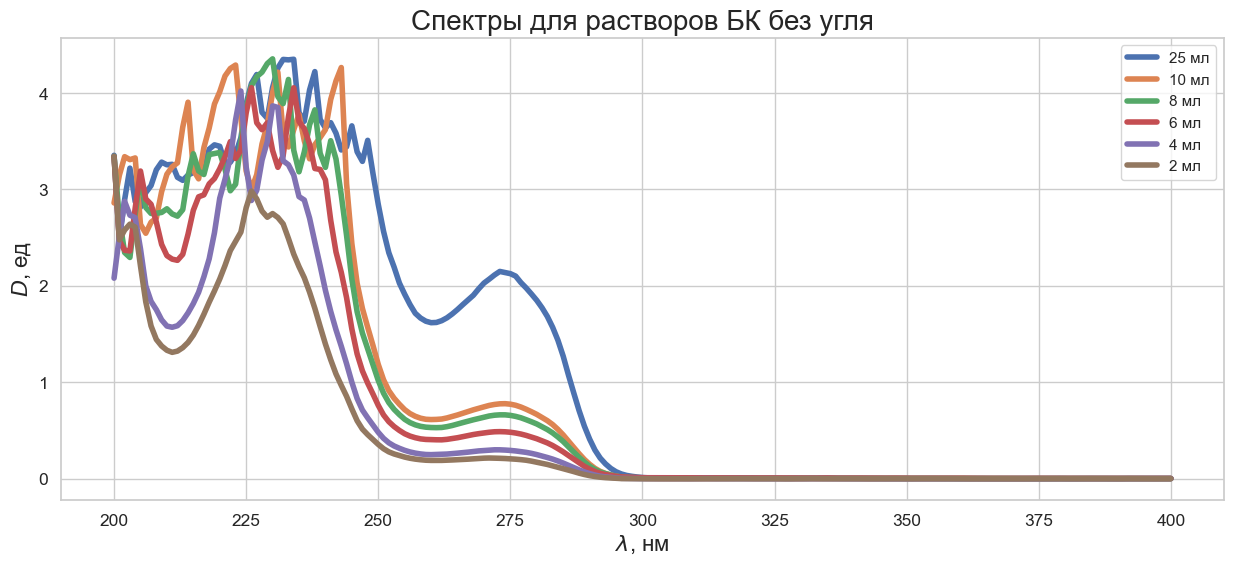
\includegraphics[width=18cm]{spectr.png}
    \caption{График зависимости оптической плотности $D$ от длины волны $\lambda$ света, проходящего через кювету с раствором БК \textbf{без угля}. В легенде указан объем концентрированной БК, который пошел на приготовление данных растворов.}
    \label{spec}
\end{figure}


При анализе графиков видно, что существует отчетливый 2-ой максимум поглощения света на длине волн $~270-275$ нм для растворов БК без угля. При этом практически незаметен максимум поглощения света на тех же участках длин волн для растворов БК с углем. 
\par
Кроме того заметим, что при длинах волн порядка 300 нм. наблюдается разная картина поглощения для двух видов растворов. Так, растворы БК без угля практически не имеют оптической плотности ($D\sim0.01$), а растворы БК с углем имеют оптическую плотность $D\sim0.1$. Так как мы предполагаем, что уголь должен быть полностью отфильтрованным из полученных растворов, то по закону \eqref{blb} на данном диапазоне длин волн для отфильтрованных растоворов с углем оптическая плотность должна получаться меньше, чем для исходных растворов. Тогда из предположения, что некоторая часть угля неотфильтровалась и поглощает вместе с оставшейся БК в растворе, можно пронормировать график по оптической плотности для длины волны 300 нм. (вычесть значение оптической плотности для длины волны 300 нм. из всего спектра). Таким образом, мы исходим из предположения, что уголь и БК уже не взаимодействуют в растворе (формула \eqref{add}) и того, что спектр поглощения угля равномерен на некотором диапазоне, хотя бы на интервале 270 - 300 нм. Тогда в результате обработки получим нормированный график спектров для раствора БК (см рис. \ref{specn}). В дальнейшем для сравнения получим изотермы как для нормированных, так и для исходных данных без нормировки.

\begin{figure}[H]
    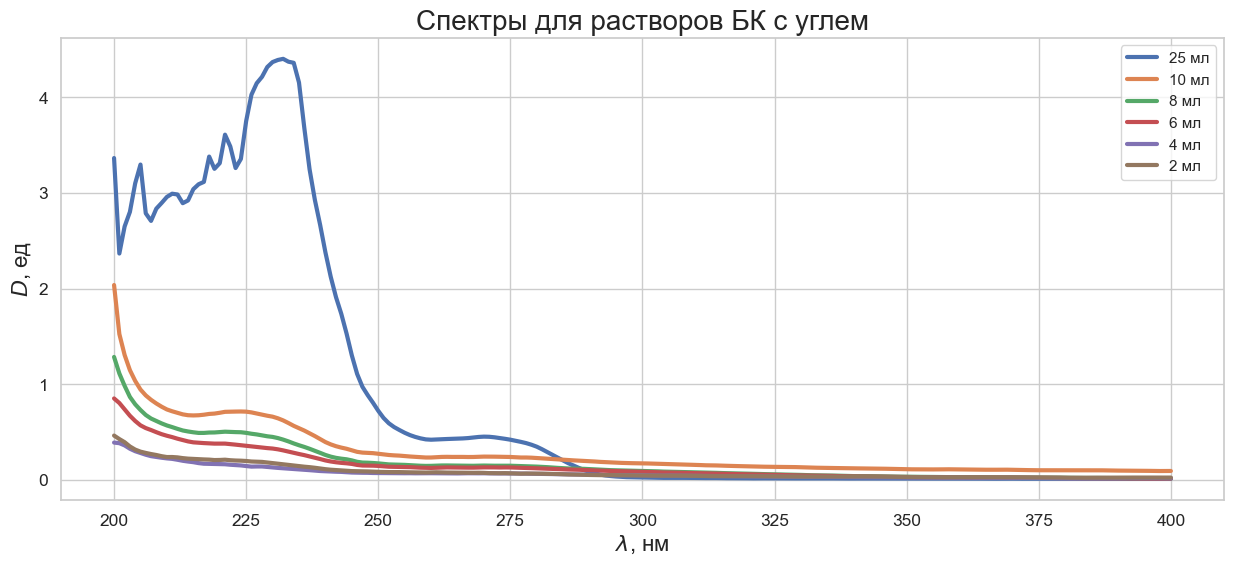
\includegraphics[width=18cm]{spectr_.png}
    \caption{График зависимости оптической плотности $D$ от длины волны $\lambda$ света, проходящего через кювету с раствором БК \textbf{с углем}. В легенде указан объем концентрированной БК, пошедший на приготовление растворов, из которых соответственно прилили изображенные на графике.}
    \label{spec_}
\end{figure}

\begin{figure}[H]
\centering
    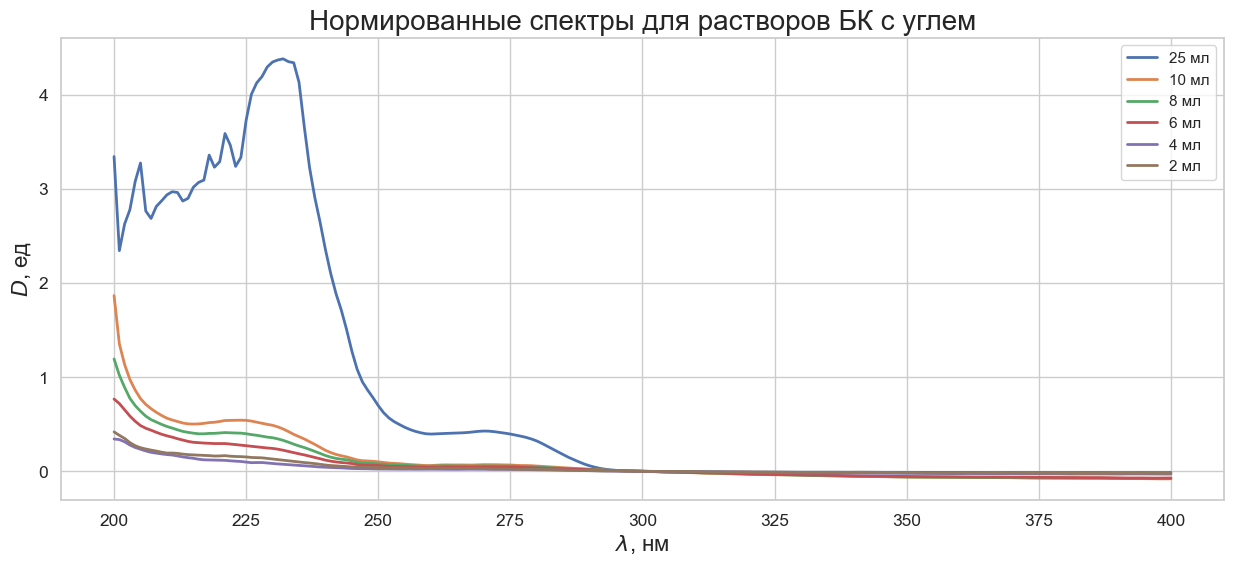
\includegraphics[width=18cm]{specn.png}
    \caption{Нормированный (на $D_0 \text{ при }  300$ нм.) график зависимости оптической плотности $D$ от длины волны $\lambda$ света, проходящего через кювету с раствором БК \textbf{с углем}. В легенде указан объем концентрированной БК, пошедший на приготовление растворов, из которых соответственно прилили изображенные на графике.}
    \label{specn}
\end{figure}

\subsection*{Изотермы адсорбций}
Из полученных спектров растворов БК без угля строим калибровочный график для нахождения коэффициента экстинкции на длине волны $\lambda$, соответствующей второму максимуму поглощения (273 нм) (см. рис. \ref{kalibr}).

\begin{figure}[H]
    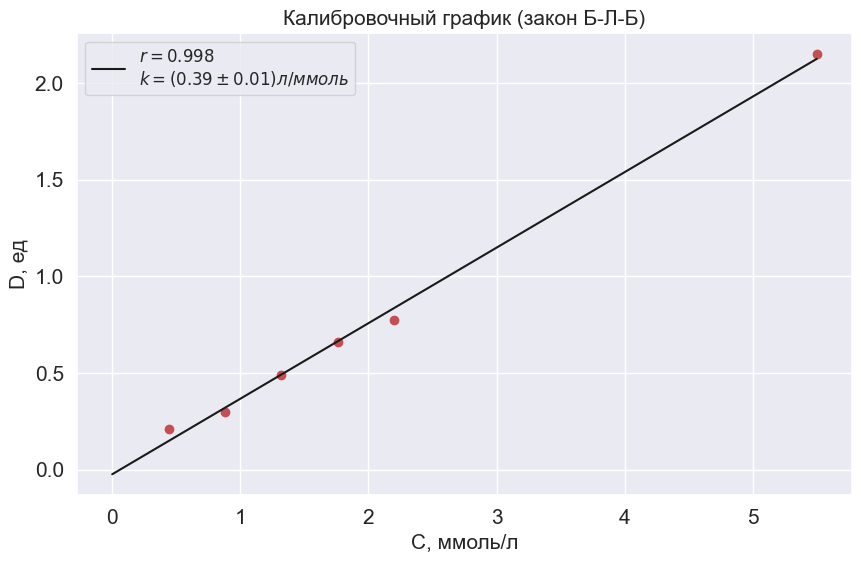
\includegraphics[width=18cm]{kalibr.png}
    \caption{Калибровочный график для получения коэффициента экстинкции, зависимость оптической плотности $D$ на длине волны 273 нм от концентрации $C_{\text{исх}}$.}
    \label{kalibr}
\end{figure}

 Затем по найденному коэффициенту экстинкции получаем концентрации растворов после адсорбции ($C_{\text{равн}}$). Далее с помощью формулы \eqref{adsorb_} найдем непосредственно величину адсорбции $\Gamma$, по которой построим соответствующие изотермы адсорбции:
\begin{equation}
    \Gamma = \dfrac{\Delta C \cdot V}{m}, \textrm{ где}
    \label{adsorb_}
\end{equation}
$\Delta C$ - разность $C_{\text{исх}}$ и $C_{\text{равн}}$, \newline $V$ - объем раствора, 
\newline $m$ - масса адсорбента
\\ Графики изотерм адсорбции см. в приложении "Данные без нормировки" и "Данные с нормировкой"



\section*{Вывод}
В данной работе с помощью измеренных спектров на спектрофотометре были получены изотермы адсорбции (Генри, Фрейндлиха и Ленгмюра) для нормированных и ненормированных данных. Для всех построенных изотерм в качестве способа проверки гипотез о линейности вычислялся коэффициент корреляции Пирсона. Для изотерм Генри и Фрейндлиха коэффициент корреляции $r > 0.9$ при учете всех 6 растворов БК. Причем для изотермы Фрейндлиха коэффициент корреляции может существенно повыситься, если не учитывать два или один из двух наименее концентрированных растворов БК. При построеннии изотерм Ленгмюра на всей выборке коэффициент корреляции был $r < 0.8$. Из-за этого данные для наименее концентрированного раствора были причислены к выбросам, как вносящие самую большую ошибку. На рисунках в приложении представлены графики изотерм Ленгмюра без учета выбросов.
\par
При сравнении изотерм, построенных для нормированных и исходных данных можно увидеть, что коэффициент корреляции практически не различает их. Однако если сравнить изотермы Генри, то мы сможем увидить различие концентраций БК в растворах: для данных без нормировки значения $C$ распределены более равномерно, и значение для наиболее концентрированного раствора не так сильно выделяется, как для данных с нормировкой.
\par
Исходя из анализа методики проведения эксперемента можно сделать вывод, что наибольший вклад в ошибку дает уголь, который остался в растворе после фильтрования. Он был виден невооруженным глазом во втором растворе, что хорошо отображается на построенных графиках. Причем факт того, что при длинах волн больше 300 нм. мы наблюдаем рост оптической плотности с 0,01 до 0,1 ед., доказывает наличия угля в отфильтрованном растворе (т.к. точность измерений спектрофотометра $\Delta D \sim 0.01 $ - см. рис. \ref{wat}). При этом данная ошибка не может быть полноценно учтена в ходе обработки, в том числе с помощью нормировки, потому что нам неизвестно как именно уголь поглощает свет, и равномерное приближение так же будет неточным. 





\section*{Приложение}
\begin{table}[H]
\centering
\begin{tabular}{|l|l|l|l|l|l|l|}
\hline
Номер раствора                                                                  & 1  & 2  & 3  & 4  & 5  & 6  \\ \hline
\begin{tabular}[c]{@{}l@{}}Объем\\  насыщенного\\  раствора БК, мл\end{tabular} & 25 & 10 & 8  & 6  & 4  & 2  \\ \hline
\begin{tabular}[c]{@{}l@{}}Объем\\ дистиллированной\\ воды, мл\end{tabular}     & 75 & 90 & 92 & 94 & 96 & 98 \\ \hline
\begin{tabular}[c]{@{}l@{}}Концентрация\\  раствора БК, мМоль/л \end{tabular} & 5.5 & 2.2 & 1.76  & 1.32  & 0.88  & 0.44  \\ \hline
\end{tabular}
\caption{Пропорции рабочих растворов.}
\label{prop}
\end{table}

\begin{table}[H]
\begin{tabular}{|l|ll|l|}
\hline
\multirow{2}{*}{\begin{tabular}[c]{@{}l@{}}Исходная\\ концентрация раствора, ммоль/л\end{tabular}} &
  \multicolumn{2}{l|}{оптическая плотность, $\lambda = 273$ нм} &
  \multirow{2}{*}{\begin{tabular}[c]{@{}l@{}}Концентрация после\\ адсорбции, ммоль/л\end{tabular}} \\ \cline{2-3}
     & \multicolumn{1}{l|}{до адсорбции} & после адсорбции &      \\ \hline
0.44 & \multicolumn{1}{l|}{0.2}          & 0.07            & 0.03 \\ \hline
0.88 & \multicolumn{1}{l|}{0.3}          & 0.07            & 0.03 \\ \hline
1.32 & \multicolumn{1}{l|}{0.5}          & 0.13            & 0.05 \\ \hline
1.76 & \multicolumn{1}{l|}{0.7}          & 0.15            & 0.06 \\ \hline
2.2  & \multicolumn{1}{l|}{0.8}          & 0.24            & 0.09 \\ \hline
5.5  & \multicolumn{1}{l|}{2.1}          & 0.4             & 0.17 \\ \hline
\end{tabular}
\caption{Результаты измерения оптической плотности растворов БК до и после адсорбции (c нормировкой)}
\end{table}

\begin{table}[H]
\begin{tabular}{|l|ll|l|}
\hline
\multirow{2}{*}{\begin{tabular}[c]{@{}l@{}}Исходная\\ концентрация раствора, ммоль/л\end{tabular}} &
  \multicolumn{2}{l|}{оптическая плотность, $\lambda = 273$ нм} &
  \multirow{2}{*}{\begin{tabular}[c]{@{}l@{}}Концентрация после\\ адсорбции, ммоль/л\end{tabular}} \\ \cline{2-3}
     & \multicolumn{1}{l|}{до адсорбции} & после адсорбции &       \\ \hline
0.44 & \multicolumn{1}{l|}{0.2}          & 0.024           & 0.009 \\ \hline
0.88 & \multicolumn{1}{l|}{0.3}          & 0.020           & 0.008 \\ \hline
1.32 & \multicolumn{1}{l|}{0.5}          & 0.04            & 0.017 \\ \hline
1.76 & \multicolumn{1}{l|}{0.7}          & 0.05            & 0.021 \\ \hline
2.2  & \multicolumn{1}{l|}{0.8}          & 0.07            & 0.03  \\ \hline
5.5  & \multicolumn{1}{l|}{2.1}          & 0.4             & 0.16  \\ \hline
\end{tabular}
\caption{Результаты измерения оптической плотности растворов БК до и после адсорбции (c нормировкой)}
\end{table}

\begin{table}[H]
\centering
\begin{tabular}{|l|l|l|}
\hline
Уравнение                   & Параметр      & Значение с указанием единиц измерений \\ \hline
\multirow{2}{*}{Генри}      & $K_H$         & 48 л/г                                \\ \cline{2-3} 
                            & $R^2$         & 0.964                                 \\ \hline
\multirow{3}{*}{Ленгмюра}   & $\text{Г}_{max}$ & 12.5 ммоль/г                          \\ \cline{2-3} 
                            & $K_L$         & 4.2 л/ммоль                           \\ \cline{2-3} 
                            & $R^2$         & 0.953                                 \\ \hline
\multirow{3}{*}{Фрейндлиха} & $K_F$         & 55                                   \\ \cline{2-3} 
                            & n             & 1.1                                   \\ \cline{2-3} 
                            & $R^2$         & 0.906                                 \\ \hline
\end{tabular}
\caption{Параметры уравнений Генри, Фрейндлиха и Ленгмюра, определенные графически (данные без нормировки)}
\end{table}

\begin{table}[H]
\centering
\begin{tabular}{|l|l|l|}
\hline
Уравнение                   & Параметр      & Значение с указанием единиц измерений \\ \hline
\multirow{2}{*}{Генри}      & $K_H$         & 43 л/г                                \\ \cline{2-3} 
                            & $R^2$         & 0.941                                 \\ \hline
\multirow{3}{*}{Ленгмюра}   & $\text{Г}_max$ & 7.7 ммоль/г                           \\ \cline{2-3} 
                            & $K_L$         & 26 л/ммоль                            \\ \cline{2-3} 
                            & $R^2$         & 0.960                                 \\ \hline
\multirow{3}{*}{Фрейндлиха} & $K_F$         & 37                                    \\ \cline{2-3} 
                            & n             & 0.73                                  \\ \cline{2-3} 
                            & $R^2$         & 0.852                                 \\ \hline
\end{tabular}
\caption{Параметры уравнений Генри, Фрейндлиха и Ленгмюра, определенные графически (с нормировкой)}
\end{table}

\begin{figure}[H]
    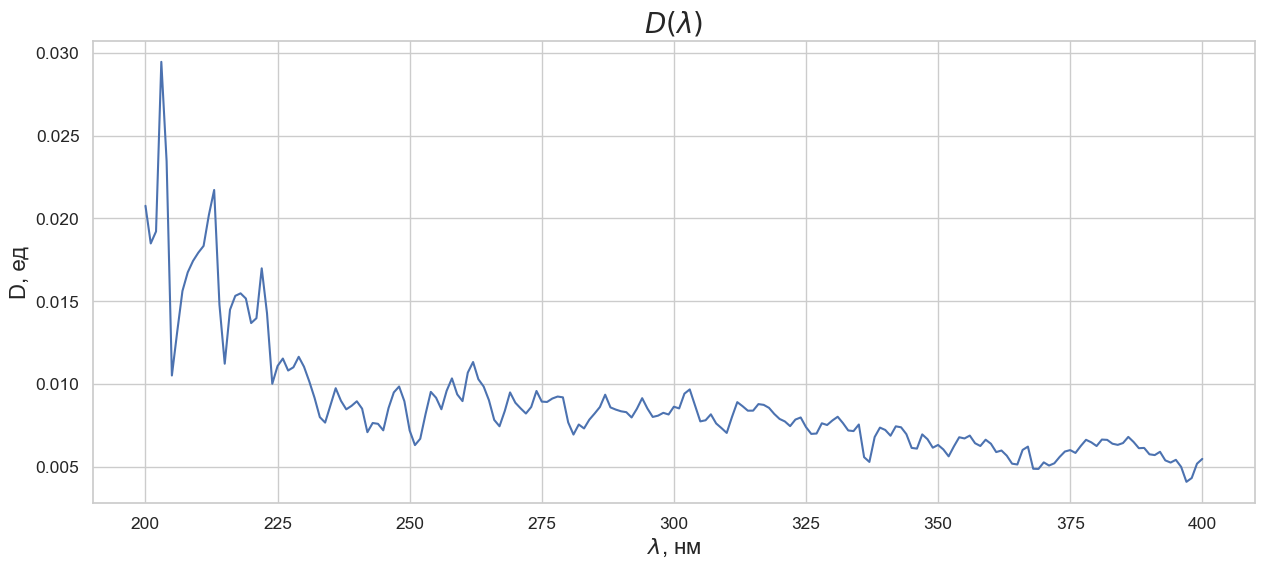
\includegraphics[width=18cm]{water.png}
    \caption{Измерение дистиллированной воды на спектрофотометре при откалиброванном "нуле" \\ спектрофотометра.}
    \label{wat}
\end{figure}


\subsection*{Данные без нормировки}

\begin{figure}[H]
    \centering
    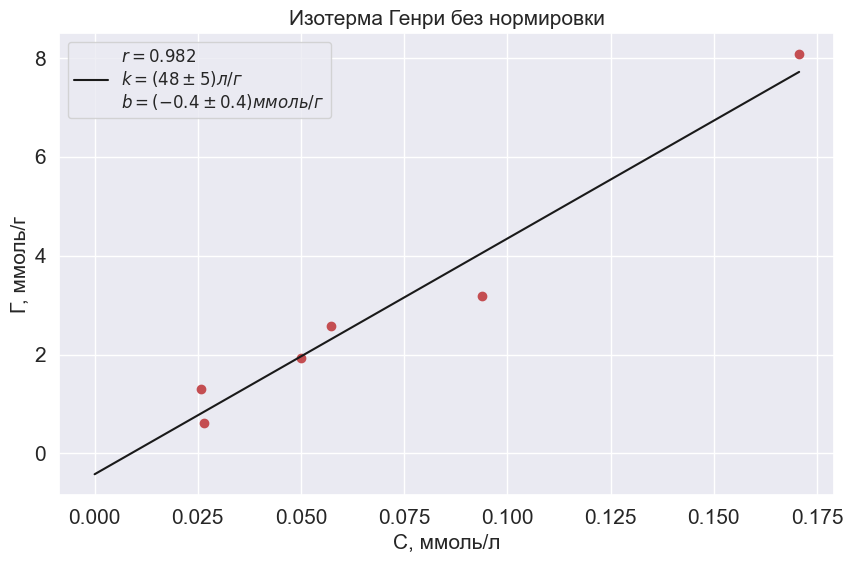
\includegraphics[width=17cm]{Henri.png}
    \label{Henri}
\end{figure}

\begin{figure}[H]
    \centering
    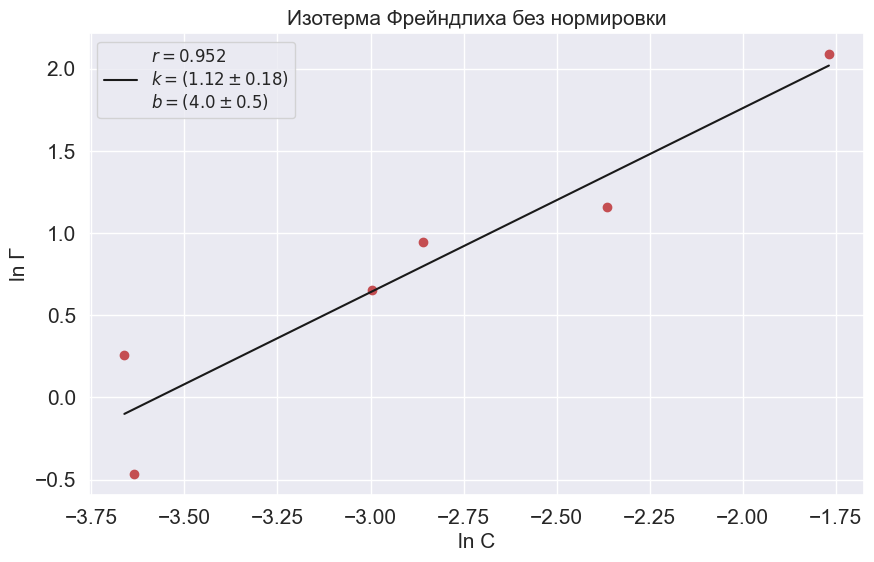
\includegraphics[width=17cm]{FR.png}
    \label{FR}
\end{figure}

\begin{figure}[H]
    \centering
    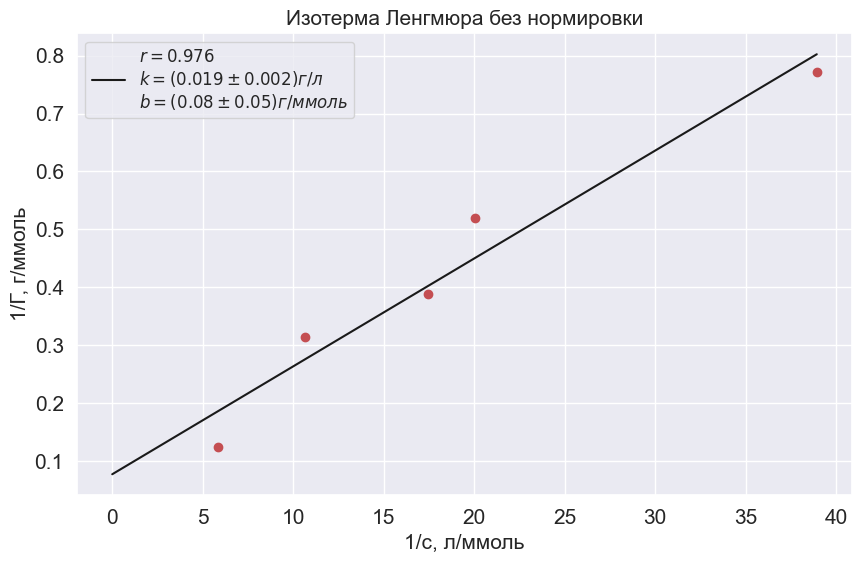
\includegraphics[width=17cm]{leng.png}
    \label{leng}
\end{figure}

\subsection*{Данные с нормировкой}

\begin{figure}[H]
    \centering
    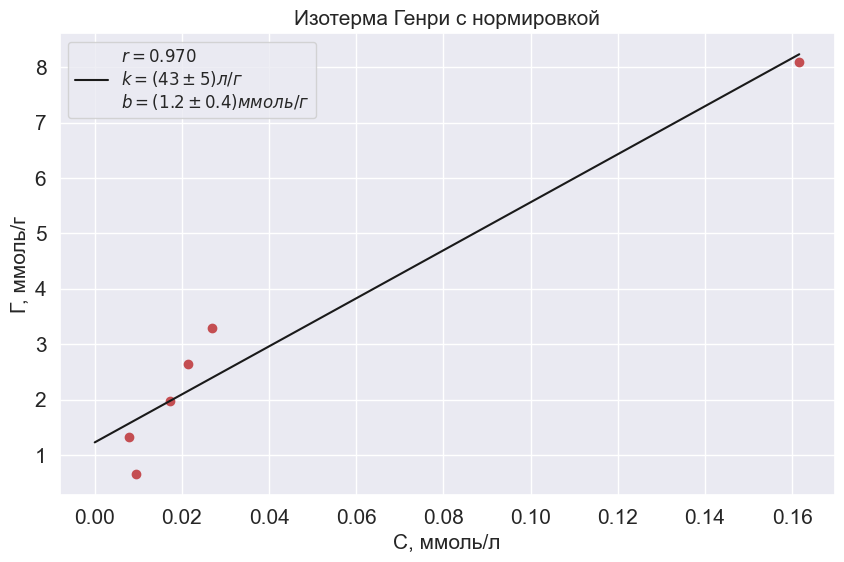
\includegraphics[width=17cm]{Henri_n.png}
    \label{Henri_n}
\end{figure}

\begin{figure}[H]
    \centering
    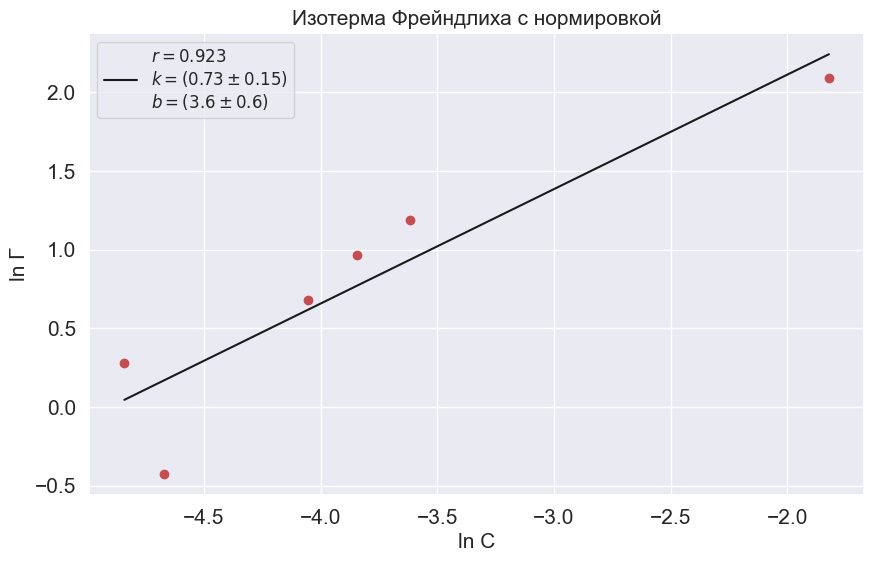
\includegraphics[width=17cm]{FR_n.png}
    \label{FR_n}
\end{figure}

\begin{figure}[H]
    \centering
    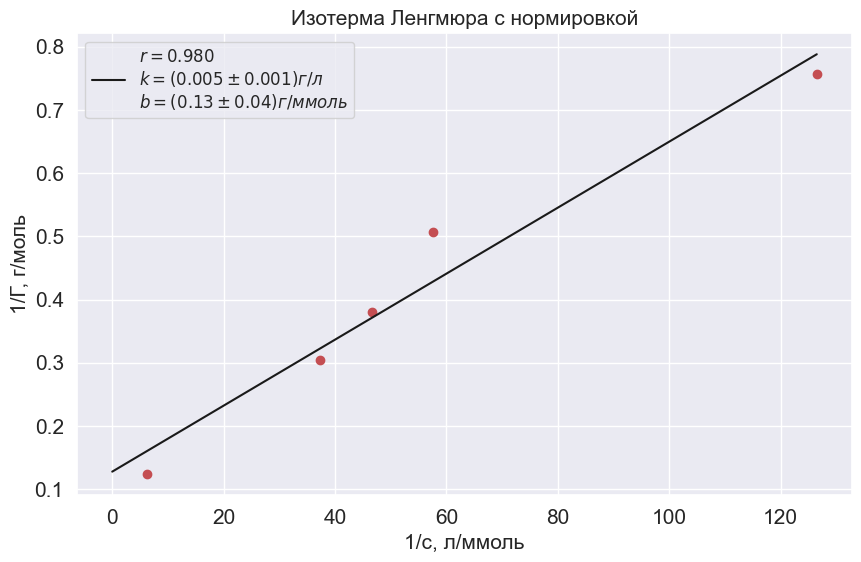
\includegraphics[width=17cm]{leng_n.png}
    \label{leng_n}
\end{figure}





\end{document}

